\section{Architecture}

\begin{figure}[t]
   \begin{center}
     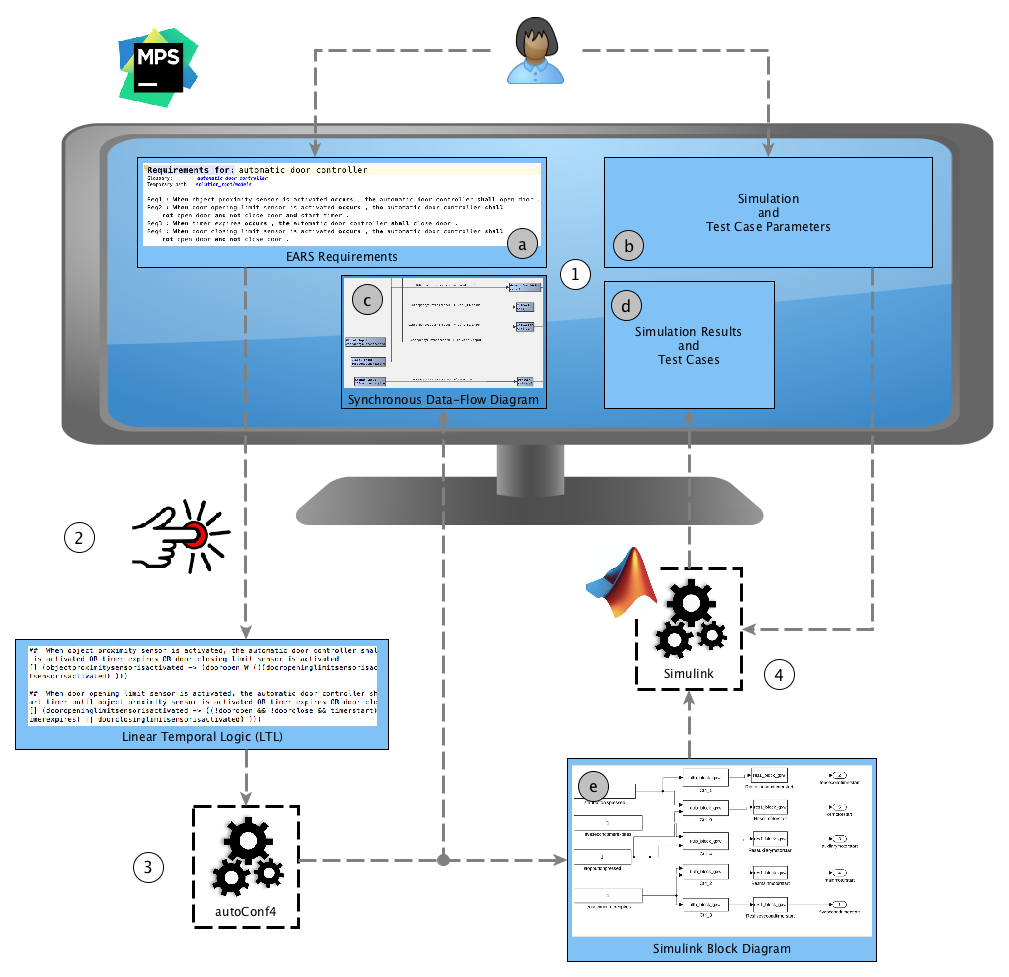
\includegraphics[width=1\textwidth]{images/toolchain.png}
     \caption{The \textsf{EARS-CTRL} Tool Chain}
     \label{fig:ears_ctrl_toolchain}
   \end{center}
 \end{figure}
 
In figure~\ref{fig:ears_ctrl_toolchain} we depict the architecture of the
\textsf{EARS-CTRL} tool. In the following paragraphs we will provide to the
reader a brief description of the main components of the tool's architecture,
how those components have been implemented and which artifacts those
components interchange. 
 
\paragraph{1. Editors and Control Panels\\\\} 

The requirements editor, the glossary editor, the simulation control panel, the
test generation control panel and the synchonous data-flow diagram visualizer
have all been built as domain-specific languages in the MPS meta-editing tool.
The languages are mostly composed of an abstract syntax (also known as
meta-model) and a concrete syntax which allows displaying and editing the
information in a clean fashion, as depicted in figures~\ref{fig:ears_reqs} and
~\ref{fig:ears_glossary}\levi{more figures?}. In order to build a new set of
requirements or a glossary the requirements engineer simply builds an instance
(also known as a model) of the corresponding language.\levi{what about the
simulation and test generation control panels?} Note that because MPS is a
projectional editor the abstract syntax is directly edited in the model. A
direct consequence of this is for example the fact that when a glossary
component's name is updated in the glossary editor, that term will be
immediately updated in any requirements that refer to that component name. This
is because requirements directly refer to the component names defined in the
glossary.

\paragraph{2. From EARS to Lineal Temporal Logic\\\\}

Let us consider the requirement \textsf{Req1} which is part of the
specification of the sliding doors controller in figure~\ref{fig:ears_reqs}:

\begin{center}
\textbf{When} \emph{object proximity sensor is activated} \textbf{then the} \emph{automatic door controller} \textbf{shall}
\emph{open door}.
\end{center}

 This requirement, taken in isolation, translates into the following LTL
 formula:
 
$$[] (objectproximitysensorisactivated \rightarrow dooropen)$$
which, if one takes into consideration the semantics of the $\rightarrow$
operator as ``implies'', is the expected logical meaning of \textsf{Req1}. All EARS
templates, when taken in isolation, can be directly translated into LTL and
propositional logic operators in such a straightforward manner.
If, however, one translates the whole set of requirements for the automatic
door in \ref{fig:ears_reqs} into LTL, the result for \textsf{Req1} will be as follows:

\begin{align*}
[] (objectproximity&sensorisactivated \rightarrow\\
 &(dooropen\,W\,(dooropeninglimitsensorisactivated \lor timerexpires\\
 & \lor doorclosinglimitsensorisactivated )))
\end{align*}

This is due to the fact that the requirements specify behaviors that are
interwined during execution. For example, from \textsf{Req1}  in
figure~\ref{fig:ears_reqs} we know that if the \textsf{object proximity sensor}
is activated, the doors will open. We also know from \textsf{Req2} that, when
the \textsf{opening limit reached} sensor is activated, the doors will stop.
Without additional information, the \textsf{autoConf4} synthesis tool identifies
a contradition in these two requirements since, if the two sensors are activated
in whichever order, the doors will simultaneously open and close. In order to
avoid such contradictions we need to establish a temporal dependence between the
behaviors specified by the requirements. In order to do so we statically analyse
the requirements and identify such dependencies in order to add this information
to the automatically generated LTL specification.
This is clear in the second translation above: the door will only open,
\emph{until} (the ``\textbf{W}'' operator) the door \textsf{opening limit
reached} sensor is activated, \emph{or} other events stated in related
requirements occur.
 
\paragraph{3. Synthesizing a Controller using \textsf{autoConf4}\\\\}

Interfacing with \textsf{autoConf4} using MPS's Java API interfacing. 

\paragraph{4. Simulation and Test Generation using Simulink\\\\}

After passing the LTL specification obtained from the \textsf{EARS-CTRL}
requirements to the the \textsf{autoConf4} synthesizer we obtain a
synchronous data-flow (SDF) diagram which, for short, consists of a set of
synchronized blocks that perform arithmetic, logical or other functions on
input signals and return the result on output signals.The controller's inputs
and outputs are also represented as specific blocks. Synchronization between
blocks is achieved by connecting those blocks' inputs and outputs via wires.
In order to simulate \textsf{EARS-CTRL} specifications we have built a
translator from such data-flow diagrams onto Simulink models. Given that the
synchronous data-flow diagram formalism is very similar to the Simulink
formalism, the structural translation is essentially one-to-one. However, only a
subset of all blocks present in SDF specifications produced by
\textsf{autoConf4} was readily available in Simulink. As such, a number of
Simulink blocks had to be built by us to accomodate the semantics of SDF
specifications. In particular\ldots\levi{add some more detail here}. 

The Simulink model is generated by \textsf{EARS-CTRL} as a text script that is
loaded into Simulink for execution. Additional Simulink scripts are generated
by \textsf{EARS-CTRL} in order to allow for test-case generation. The whole is
glued and orchestrated by \textsf{EARS-CTRL} using system calls.\levi{how is
step-by-step simulation done?}
